% "{'classe':('PSI'),'chapitre':'slci_pi','type':('td'),'titre':'Agitateur médical avec chambre de Riccordi', 'source':' CCP - PSI - 2006','comp':('C1-02','C2-04'),'corrige':True}"
%\setchapterimage{bandeau}
\chapter*{TD \arabic{cptTD} \\ 
Agitateur médical avec chambre de Riccordi -- 
\ifprof Corrigé \else Sujet \fi}
\addcontentsline{toc}{section}{TD \arabic{cptTD} :
Agitateur médical avec chambre de Riccordi -- 
\ifprof Corrigé \else Sujet \fi}

\iflivret \stepcounter{cptTD} \else
\ifprof  \stepcounter{cptTD} \else \fi
\fi

\setcounter{question}{0}
\marginnote{CCP -- PSI -- 2006.}
%\marginnote[1cm]{
%\UPSTIcompetence[2]{C1-02}
%\UPSTIcompetence[2]{C2-04}}
\marginnote{\xpComp{COR}{02}\xpComp{COR}{03}}

\begin{marginfigure} [4cm]
\centering
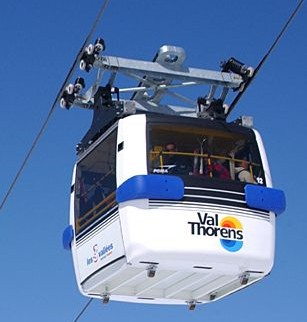
\includegraphics[width=\linewidth]{fig_00}
\end{marginfigure}



\subsection*{Présentation}

%\noindent\begin{minipage}[c]{.6\linewidth}

Afin d'isoler des cellules issues du pancréas, il est nécessaire de les baigner dans un mélange d'enzymes tout en agitant la solution dans un milieu contrôlé en température. On utilise pour cela 
un agitateur médical avec chambre de Riccordi.


\begin{obj}
La maîtrise de la température joue un rôle crucial, l’objectif de notre étude est de réduire les temps
de réaction et d’augmenter la précision en température du système de chauffage. Le cahier des charges est le suivant : 
\begin{itemize}
\item temps de montée en température : \SI{3}{min} maxi;
\item précision de la température : $\pm \SI{0,5}{\degres}$ pour un échelon de $\SI{20}{\degres}$.
\end{itemize}
\end{obj}
Nous utilisons pour chauffer la solution circulant dans la chambre, un collier chauffant situé sur le
pourtour de la chambre, alimenté en tension par une unité comprenant un correcteur et un
amplificateur.

%Cette unité élabore une tension, dépendant de la tension de consigne fournie par un appareillage
%auxiliaire $U_{tc}$ (non étudié dans cette étude) et de la tension $U_t$ provenant d'un capteur de température
%situé dans la chambre.



On note : 
\begin{itemize}
\item $U_{tc}$ : tension de consigne;
\item $U_t$ : tension à l'image de la température (capteur de température mesurant la température dans la chambre);
\item $U_a$ : tension d'alimentation du collier chauffant;
\item $q_c$ : énergie calorifique fournie par le collier chauffant;
\item $q_p$ : énergie calorifique perdue ou reçue par la chambre (en dehors du collier chauffant) perte par convection, par circulation de l'enzyme. Dans le cadre de cette étude \textbf{on néglige les pertes}.
\end{itemize}

\begin{center}
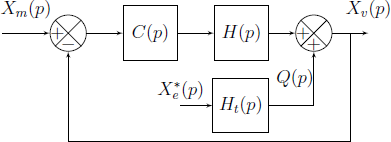
\includegraphics[width=\linewidth]{fig_03}
%\textit{}
\end{center}
%
%\question{Expliquez la signification du sommateur situé, sur le schéma-blocs, en amont du bloc transfert de la chambre.}
%
%
%\subsection*{Identification du système}
%On ouvre la boucle de régulation en ne gardant que l'amplificateur, le collier chauffant, la chambre et le capteur de température.
%
%\begin{center}
%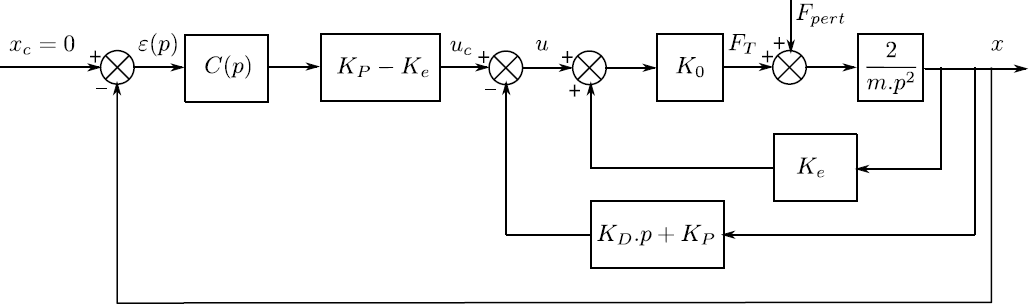
\includegraphics[width=\linewidth]{fig_02}
%%\textit{}
%\end{center}
%
%Le système est stabilisé à 17\degres C avec une tension $U_c=\SI{0}{V}$. Le capteur de température est calibré pour
%fournir une tension de \SI{0}{V} à cette température.
%On applique brusquement une tension de \SI{10}{V} à l'entrée de l'amplificateur. On relève à l'aide du
%capteur de température l'augmentation de température (valeur de tension en sortie du capteur de température $U_t$).

Expérimentalement, on peut déterminer que $\text{FTBO(p)}=\dfrac{U_t(p)}{U_c(p)}=\dfrac{0,5}{\left(1+5 p \right)\left(1+100 p \right)}$.

\subsection*{Analyse des performances}
On considère ici que $C(p)=1$. On donne l'abaque des temps de réponse réduit plus bas.


\question{Déterminer le temps de réponse à 5\% du système régulé.}

\question{Déterminer l'écart en position et l'écart en traînage.}

\question{Justifier le tracé du diagramme de Bode de la FTBO non corrigée (figure \ref{Cy_03_01_TD_PI_02_bode})}


\ifprof
\else
\begin{figure}[!h]
\centering
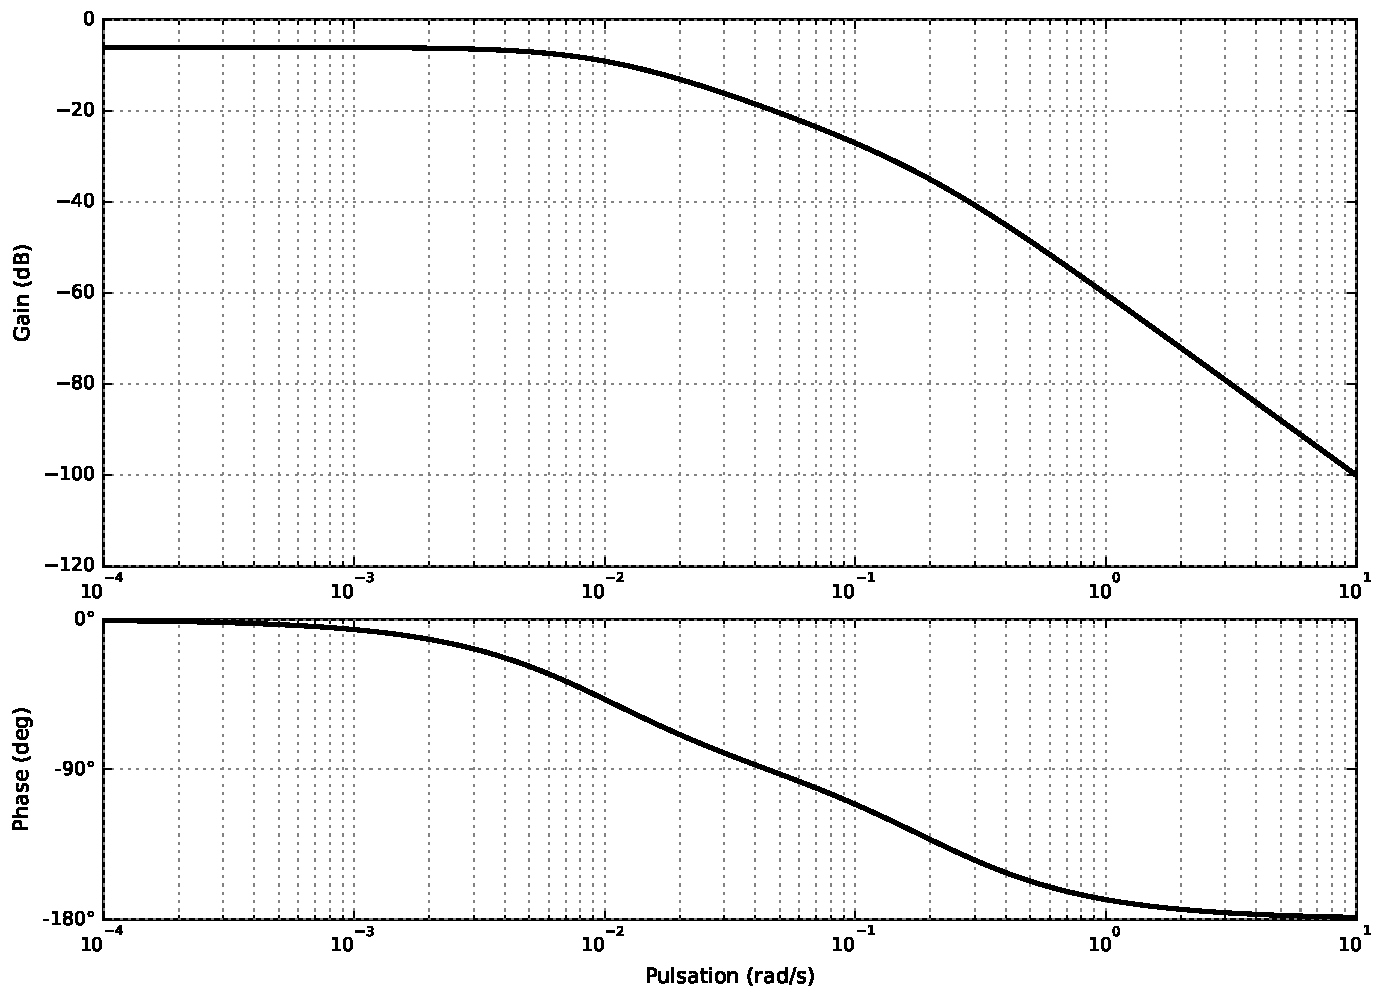
\includegraphics[width=.9\linewidth]{Bode_FTBO_NC}
\caption{Diagramme de Bode de la BO non corrigée\label{Cy_03_01_TD_PI_02_bode} }
\end{figure}
\fi


\question{Déterminer la marge de gain et la marge de phase.}

\subsection*{Mise en \oe{}uvre de corrections P et PI}

On envisage une première correction en utilisant un correcteur proportionnel de la forme $C(p)=K$.


\begin{marginfigure}
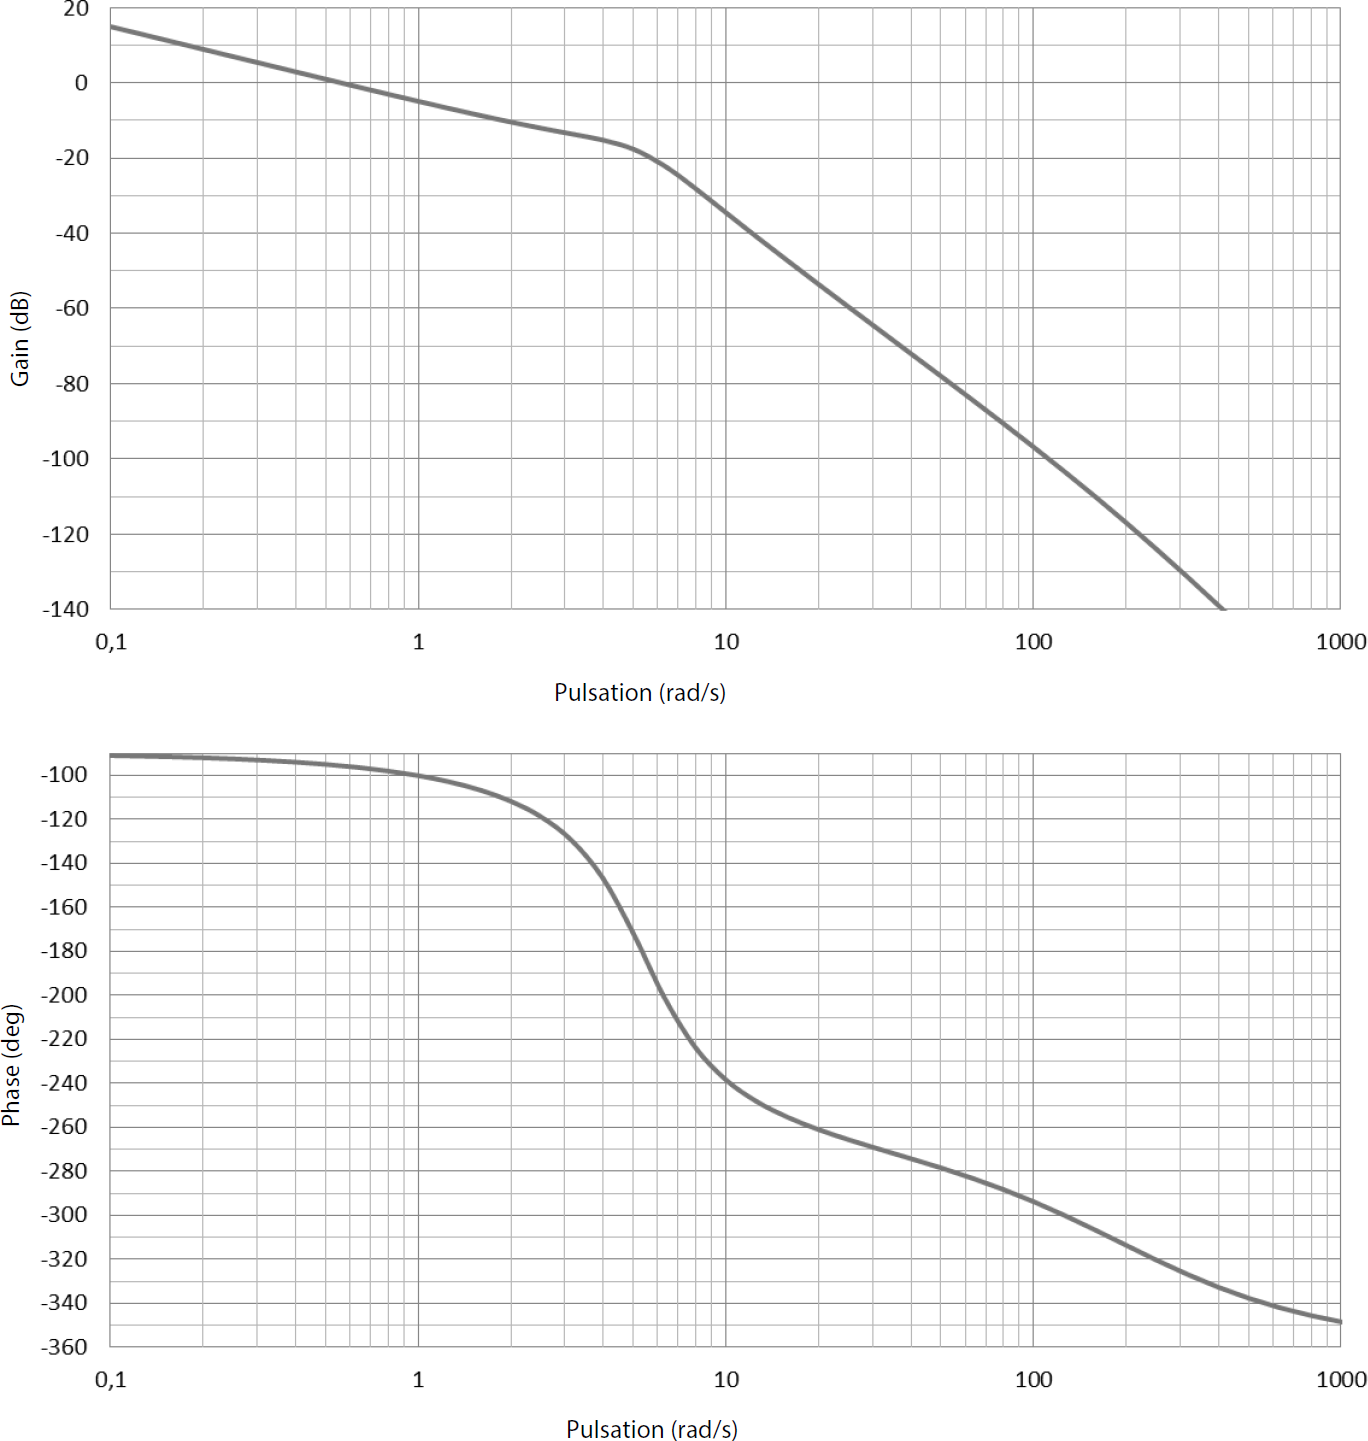
\includegraphics[width=\linewidth]{fig_04}
%%\textit{}
\end{marginfigure}

\question{Déterminer le gain $K$ de manière à obtenir le système le plus rapide sans aucun dépassement.}


\question{En déduire le temps de réponse à 5\%, l'écart en position et l'écart de traînage.}

\question{Déterminez alors, la tension en sortie de l'amplificateur , si on envoie un échelon de tension de consigne $U_{\text{tc}}$ de \SI{5}{V}. Le gain de l'amplificateur étant de 10, critiquez vos résultats.}

On souhaite maintenant corriger le système avec en utilisant une action proportionnelle intégrale $C(p)=\dfrac{K}{T_i p}\left( 1+T_i p\right)$. On utilise pour cela la méthode des compensation de pôles. 

\question{Déterminer les gain $K$ et $T_i$ permettant d'assurer le non dépassement de la consigne ainsi que le temps de réponses du système.}


\question{En déduire le nouvel écart de position.}
%\question{\'A l'aide du tracé expérimental du document réponse « Réponse indicielle et Zoom »
%qui correspond à l'augmentation de tension $U_t$ en sortie du capteur de température, identifier la
%fonction de transfert du système en Boucle ouverte défini par le rapport $\text{FTBO(p)}=\dfrac{U_t(p)}{U_c(p)}$. On pourra utiliser la forme suivante : $\dfrac{G}{\left(1+\tau_1 p \right)\left(1+\tau_2 p \right)}$.}

\ifprof
\else
\begin{marginfigure}
\centering

\includegraphics[width=3cm]{Cy_03_01_TD_PI_02_Agitateur_qr}
\end{marginfigure}
\fi

\ifprof
\else
\ifcolle
\else
\marginnote{
\begin{solution}
\begin{enumerate}
\item \SI{218}{s}.
\item $\varepsilon_P = \dfrac{1}{1+G_{\text{FTBO}}}$ et $\varepsilon_v =\infty$.
\item .
\item Système stable (FTBO ordre 2 et critère du Revers respecté) ($M_G \to \infty$, $M_{\varphi}$ non définie).
\item $K=9$.
\item \SI{50}{s}, \item $\varepsilon_P = \dfrac{1}{1+G_{\text{FTBO}}}$ et $\varepsilon_v =\infty$.
\item $U_a =\SI{450}{V}$.
\item $K=10$ et $T_i = \SI{100}{s}$.
\item $\varepsilon_P =0$.
\end{enumerate}
\end{solution}}

\fi
\fi



\ifprof
\begin{center}
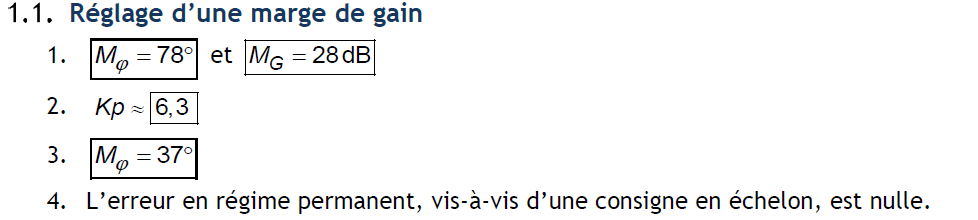
\includegraphics[width=\linewidth]{cor_01}
%%\textit{}
\end{center}
\begin{center}
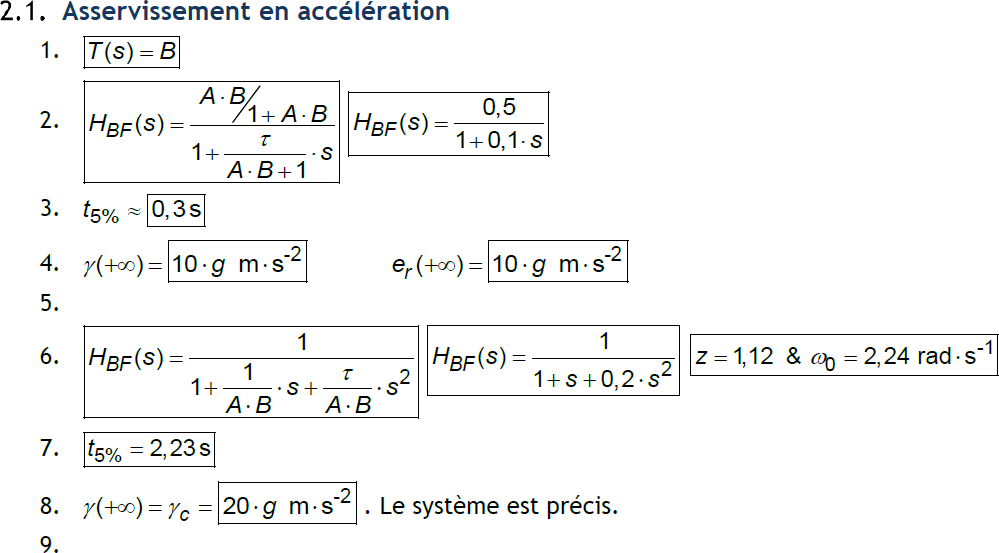
\includegraphics[width=\linewidth]{cor_02}
%%\textit{}
\end{center}
\begin{center}
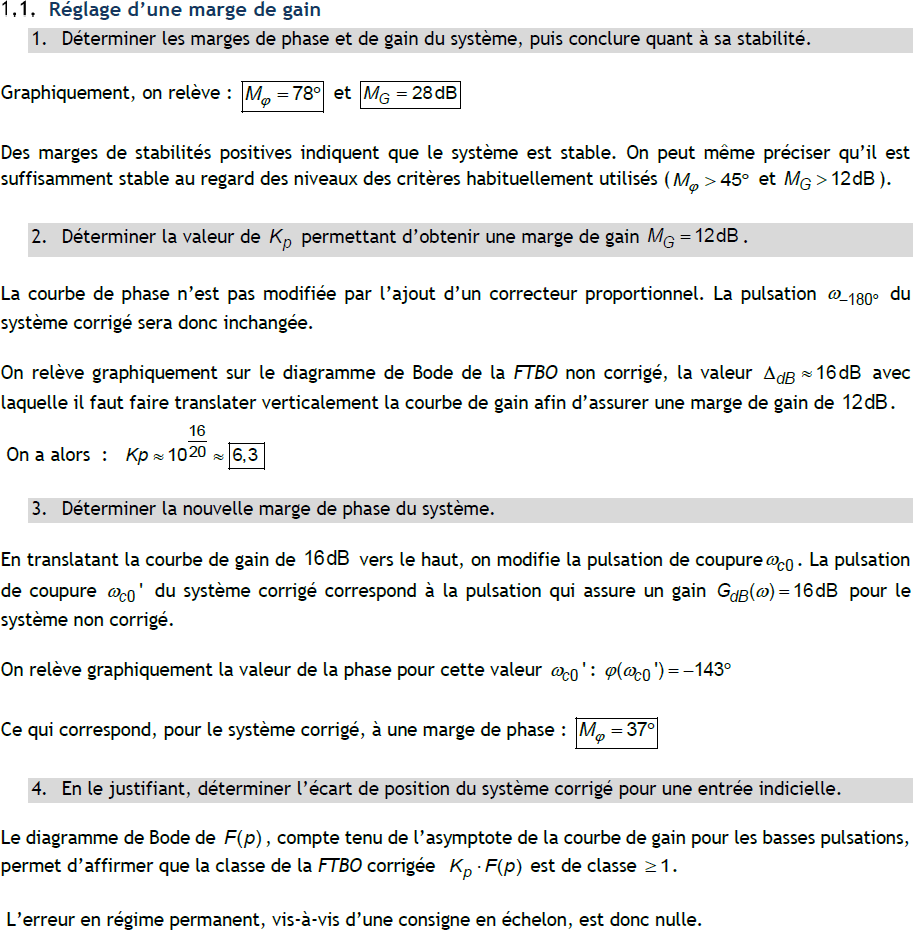
\includegraphics[width=\linewidth]{cor_03}
%%\textit{}
\end{center}
\begin{center}
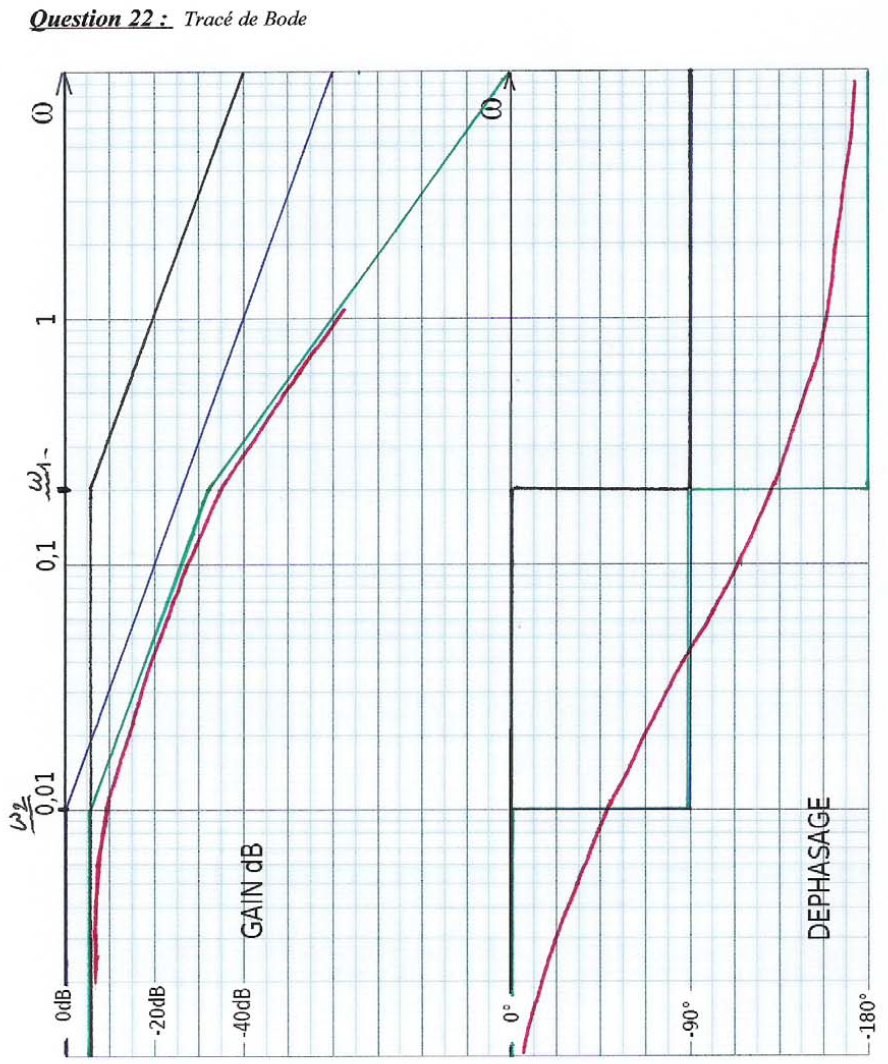
\includegraphics[width=\linewidth]{cor_04}
%%\textit{}
\end{center}
\begin{center}
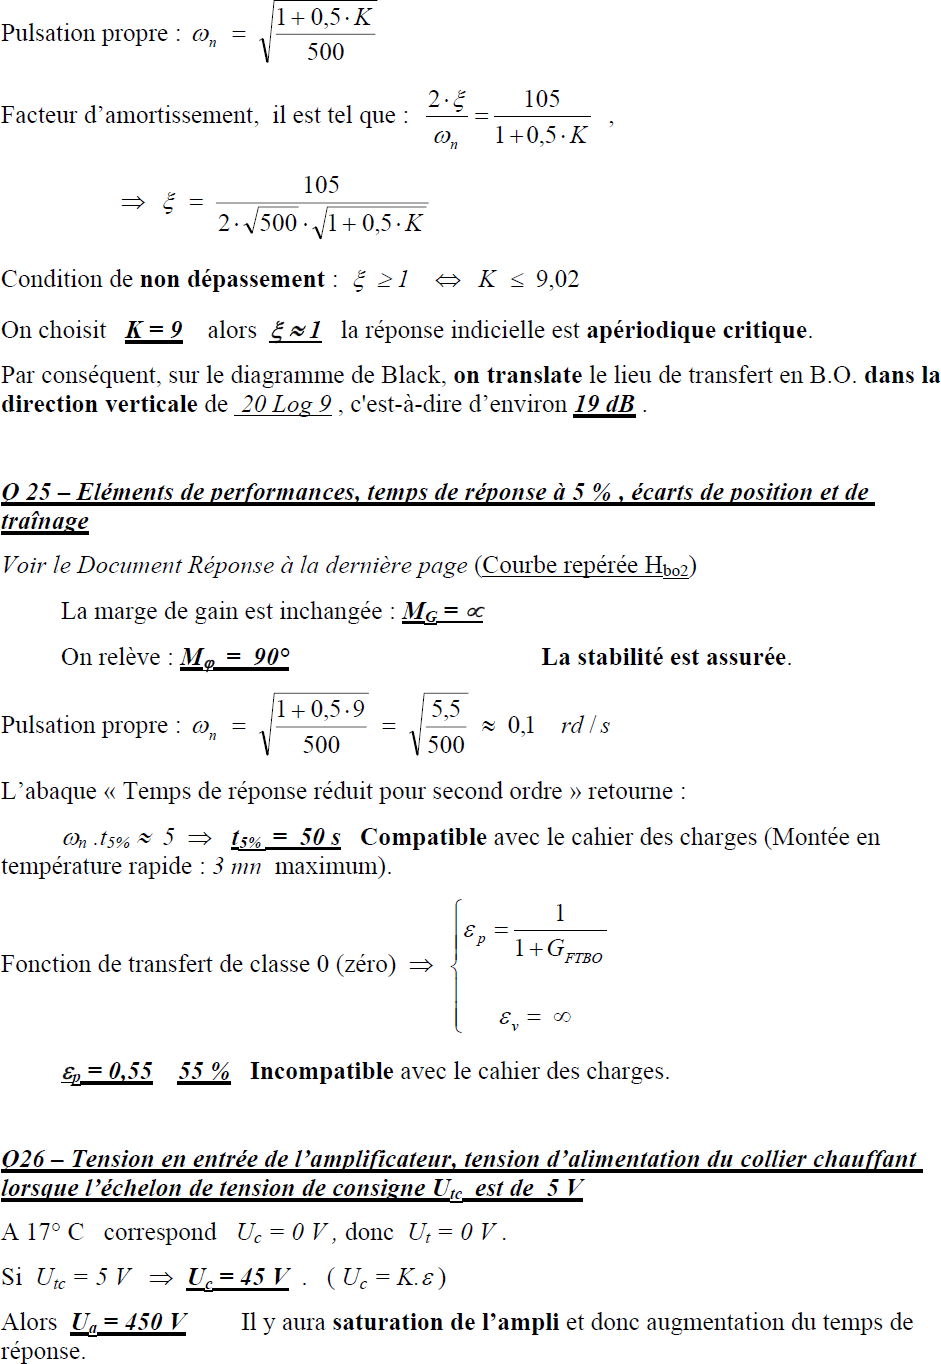
\includegraphics[width=\linewidth]{cor_05}
%%\textit{}
\end{center}
\begin{center}
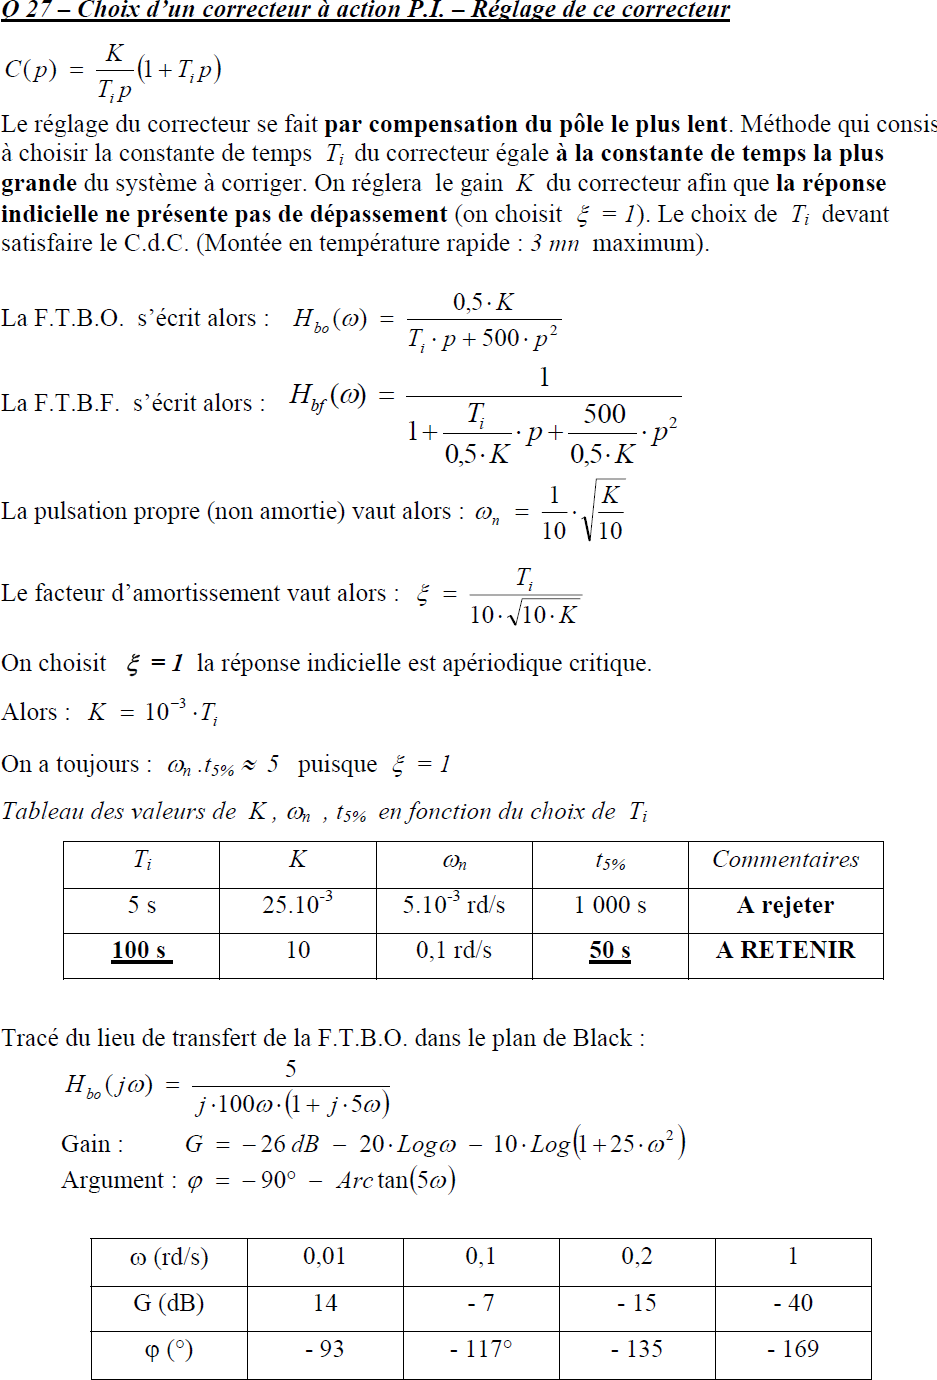
\includegraphics[width=\linewidth]{cor_06}
%%\textit{}
\end{center}
\begin{center}
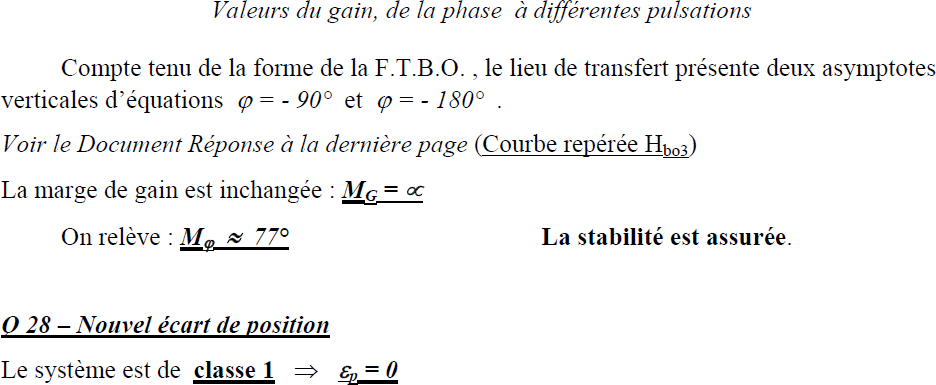
\includegraphics[width=\linewidth]{cor_07}
%%\textit{}
\end{center}
\else
\fi
